\Subsection{Голоморфные функции}

Если доказательство не указано, то оно повторяет то, что было в $\mathbb{R}$ (смотреть 1 семестр).

\begin{definition}
    $\Omega$ -- обсласть в $\mathbb{C}, \ f: \Omega \rightarrow \mathbb{C}, \ z_0 \in \Omega$.

    $f$ -- голоморфна в точке $z_0$, если существует $\lim_{z \rightarrow z_0} { \frac{f(z) - f(z_0)}{z - z_0} } =: f'(z_0)$.
\end{definition}
\begin{definition}
    $f$ комплексно дифф. в точке $z_0$, если $\exists k \in \mathbb{C}$:

    $f(z) = f(z_0) + k (z - z_0) + o(z - z_0)$ при $z \rightarrow z_0$.
\end{definition}

\begin{statement}
    $f$ -- голоморфна в точке $z_0 \Leftrightarrow f$ комплексно дифф. в точке $z_0$ и $k = f'(z_0)$.
\end{statement}

\begin{consequence}
    $f$ и $g$ голоморфны в точке $z_0$. Тогда 

    \begin{enumerate}
        \item {
            $f \pm g$ голом. в точке $z_0$
        }
        \item {
            $f \cdot g$ голом. в точке $z_0$
        }
        \item {
            Если $g(z_0 \not = 0)$, то $\frac{f}{g}$ голом. в точке $z_0$.
        }
        \item {
            Если $h$ голом. в точке $f(z_0)$, то $h \circ f$ голом. в точке $z_0$.
        }
    \end{enumerate}
\end{consequence}

\begin{remark}
    $f: \Omega \rightarrow \mathbb{C}$

    $z = x + iy, \ f(z) = f(x + iy) = g(x + i y) + i h(x + iy): \ g, h : \Omega \rightarrow \mathbb{R}$.

    $\frac{\partial f}{\partial x} (z_0) = \lim_{h \rightarrow 0, \ h \in \mathbb{R}} {\frac{f(z_0 + h) - f(z_0)}{h}} = f'(z_0)$.

    
    $\frac{\partial f}{\partial y} (z_0) = \lim_{h \rightarrow 0, \ h \in \mathbb{R}} {\frac{f(z_0 + i h) - f(z_0)}{h}} = \frac{f'(z_0)}{i} = i \cdot f'(z_0)$.
\end{remark}

\begin{remark}
    $\binom{g(x + iy)}{h(x + iy)} = \binom{g(x_0 + i y_0)}{h(x_0 + iy_0)} + \binom{a \ b}{c \ d} \binom{x - x_0}{y - y_0} + o(|| (x - x_0, y - y_0) ||)$.

    $k = \alpha + i \beta$

    $k \cdot (z - z_0) = (\alpha + i \beta) ( (x - x_0) + i (y - y_0)) = \alpha(x - x_0) - \beta(y - y_0) + i (\beta (x - x_0) + \alpha (y - y_0))$

    Вещественная линейность + $\binom{\alpha \ -\beta}{\beta \ \alpha} \Leftrightarrow$ комплескная линейность.
\end{remark}


% TODO: где-то есть места, где я пишу `\pi` и при этом забыто `\cdot i`, то есть надо `\pi \cdot i`. Это критическая ошибка, ее надо исправить !!!

\begin{remark}
    Комплескная дифференцируемость $\Leftrightarrow$ вещественная дифференцируемость + матрица Якоби $\binom{\alpha \ \beta}{-\beta \ \alpha}$

    
    Комплескная дифференцируемость $\Leftrightarrow$ вещественная дифференцируемость + условия Коши-Римана $
    \begin{cases}
        \frac{\partial Re(f)}{\partial x} = \frac{\partial Im (f)}{\partial y} \\ 
        \frac{\partial Re(f)}{\partial y} = -\frac{\partial Im (f)}{\partial x} \\ 
    \end{cases}
    $
\end{remark}
\begin{remark}
    $f(z) = f(z_0) + \underbrace{k}_{\in \mathbb{C}} (z - z_0) + o(z - z_0)$

    $k (z - z_0) = k w = |k| \cdot e^{i \phi} \cdot w, \ \phi = arg(k)$
\end{remark}


\begin{remark}
    Обозначения.

    $\frac{\partial}{\partial z} = \frac{1}{2} \cdot \left( \frac{\partial}{\partial x} - i \frac{\partial}{\partial y} \right)$
    
    $\frac{\partial}{\partial \overline{z}} = \frac{1}{2} \cdot \left( \frac{\partial}{\partial x} + i \frac{\partial}{\partial y} \right)$

    $dz = dx + i dy$

    $d \overline{z} = dx - i dy$

    $df = \frac{\partial f}{\partial x} \cdot dx + \frac{\partial f}{\partial y} dy = \frac{\partial f}{\partial z} dz + \frac{\partial f}{\partial \overline{z}} d \overline{z}$
\end{remark}

\begin{theorem}
    \textbf{Условия Коши-Римана}.

    $f: \Omega \rightarrow \mathbb{C}, \ a \in \Omega$

    $f$ -- дифф. в точке $a$ как функция из $\mathbb{R}^2$ в $\mathbb{R}^2$. Следующие условия равносильны:

    \begin{enumerate}
        \item {
            $f$ -- голоморфна в точке $a$.
        }
        \item {
            $d_a f$ -- комплексно линеен
        }
        \item {
            условия Коши-Римана
        }
        \item {
            $\frac{\partial f}{\partial \overline{z}} (a) = 0$
        }
    \end{enumerate}
\end{theorem}

\begin{proof}
    Мы выяснили все, кроме $(3) \Leftrightarrow (4)$:

    $\frac{\partial f}{\partial \overline{z}} = 0 \Leftrightarrow \frac{\partial f}{\partial x} + i \frac{\partial f}{\partial y} = 0 \Leftrightarrow \frac{\partial (Re(f) + i Im(f))}{\partial x} + i \cdot \frac{\partial (Re (f) + i Im (f))}{\partial y} = 0 \Leftrightarrow \begin{cases}
        \frac{\partial Re(f)}{\partial x} - \frac{\partial Im (f)}{\partial y} = 0 \\ 
        \frac{\partial Im(f)}{\partial x} + \frac{\partial Re(f)}{\partial y} = 0
    \end{cases}$ -- а это и есть условия Коши-Римана.
\end{proof}

\begin{remark}
    Обозначения.

    $f \in H(\Omega) \Leftrightarrow f : \Omega \rightarrow \mathbb{C}$ и голоморфна во всех точках из $\Omega$.
\end{remark}
\begin{consequence}
    $\Omega$ -- область, $f \in H(\Omega)$ и $Im(f) = const \implies f = const$
\end{consequence}
\begin{proof}
    $\frac{\partial Im (f)}{\partial y} = 0 \implies \frac{\partial Re(f)}{\partial x} = 0$

    $\frac{\partial Im (f)}{\partial x} = 0 \implies \frac{\partial Re(f)}{\partial y} = 0$

    $\implies Re(f) = const$
\end{proof}
\begin{theorem}
    \textbf{Коши} (ah, shit, here we go again...)

    $f \in H(\Omega) \implies $ форма $f(z) dz$ локально точная.
\end{theorem}
\begin{proof}
    Будет два разных док-ва.

    \begin{enumerate}
        \item {
            Для случая непрерывно-дифф. $\frac{\partial Re(f)}{\partial x}, \dots$ (имеются в виду все частные производные).

            Тогда замкнутость $\implies$ локальная точность.

            $f(z) dz = f(z) (dx + i dy) = (Re(f) + i \cdot Im(f)) \cdot (dx + i dy) = Re(f) dx - Im(f) dy + i (Im (f) dx + Re(f) dy)$.

            $P dx + Q dy$ -- замкн. $\Leftrightarrow \frac{\partial P}{\partial y} = \frac{\partial Q}{\partial x}$

            $Re(f) dx - Im(f) dy$ -- замкн. $\Leftrightarrow \frac{\partial Re(f)}{\partial y} = - \frac{\partial Im(f)}{\partial x}$

            $Im(f) dx + Re(f) dy$ -- замкн. $\Leftrightarrow \frac{\partial Im(f)}{\partial y} = \frac{\partial Re(f)}{\partial x}$
        }
        \item {
            Общий случай.

            Надо доказать, что интеграл по любому прямоугольнику со сторонами параллельными осям координат из шарика $U \subset \Omega$, содержащего произвольную точку, равен 0.

            От противного: пусть нашелся прямоугольник $P$, т.ч. $\alpha (P) := \int_P {f(z) dz } \not = 0$.

            \begin{center}
                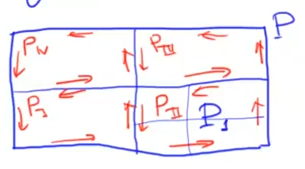
\includegraphics[width=7cm]{assets/04-functions-of-complex-variables/Cauchy-theorem-rectangle-partition.png}
            \end{center}

            
            Режем прямоугольник на 4 части, индексируем как $P^{1}, P^{2}, P^{3}, P^{4}$, строим обходы каждого (против часовой стрелки). Тогда $\alpha(P) = \alpha(P^{1}) + \alpha(P^{2}) + \alpha(P^{3}) + \alpha(P^{4})$, $|\alpha(P)| \leq |\alpha(P^{1})| + |\alpha(P^{2})| + |\alpha(P^{3})| + \alpha(P^{4})$.

            Хотя бы одно из слагаемых $\geq \frac{1}{4} |\alpha(P)|$, назовем такое $P_1$ (индекс уже снизу!). Разрежем его на 4 равные части. Пусть $P_2$ такой, что $|\alpha(P_2)| \geq \frac{1}{4} |\alpha (P_1)|$ и т.д.

            $|\alpha(P_n)| \geq \frac{1}{4^n} |\alpha (P)|$.

            % todo: picture
            \begin{center}
                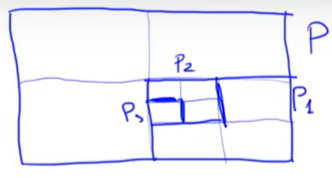
\includegraphics[width=7cm]{assets/04-functions-of-complex-variables/Cauchy-theorem-rectangle-partition-2.png}
            \end{center}

            Берем $a$ из $P_n$:

            $f(z) = f(a) + f'(a) (z - a) + o(z - a)$

            $\alpha (P_n) = \int_{P_n} { f(z) dz } = \underbrace{\int_{P_n} { f(a) dz }}_{= 0 \text{, по 1-ому док-ву}} + \underbrace{\int_{P_n} { f'(a) (z - a) dz }}_{= 0 \text{, по 1-ому док-ву}} + \int_{P_n} { o(z - a) dz }$


            \begin{center}
                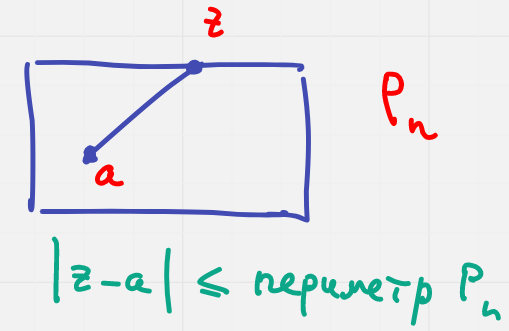
\includegraphics[width=7cm]{assets/04-functions-of-complex-variables/Cauchy-theorem-rectangle-partition-3.png}
            \end{center} 


            $o(z - a) = (z - a) \cdot \beta (z - a)$, где $\beta(z - a) \underbrace{\rightarrow}_{z \rightarrow a} 0$

            $\left| \int_{P_n} {(z - a) \beta (z - a) dz} \right| \leq max_{z \in P_n} { |z - a| \cdot |\beta (z - a)| } \cdot \underbrace{l(P_n)}_{\text{периметр}} \leq max_{z \in P_n} { |\beta (z - a)| } \cdot \frac{l(P)}{2^n} \cdot \frac{l(P)}{2^n} \implies$

            $\implies \frac{|\alpha (P)|}{4^n} \leq |\alpha(P_n)| \leq \frac{l(P) \cdot l(P)}{4^n} \cdot max_{z \in P_n} |\beta (z - a)| \implies max_{z \in P_n} |\beta (z - a)| \geq \frac{|\alpha (P)|}{l(P) \cdot l(P)} > 0$ -- противоречие, т.к. $\beta(z) \rightarrow 0$ при $z \rightarrow a$.
        }
    \end{enumerate}
\end{proof}
\begin{consequence}
    \begin{enumerate}
        \item {
            Если $f \in H(\Omega)$, то у каждой точки $a \in \Omega$ есть окрестность, в которой существует ф-я $F$, т.ч. $F' = f$ в этой окрестности.

            \begin{proof}
                Пусть $F$ первообразная формы $f(z) dz$. Поймем, что $F' = f$.

                $\frac{\partial F}{\partial x} = f(z), \ \frac{\partial F}{\partial y} = i \cdot f(z) \implies \frac{\partial F}{\partial x} + i \frac{\partial F}{\partial y} = 0 \implies \frac{\partial F}{\partial \overline{z}} = 0$
            \end{proof}
        }
        \item {
            $f \in H(\Omega)$, $\gamma$ стягиваемый в $\Omega$ путь $\implies \int_{\gamma} { f(z) dz } = 0$
        }
    \end{enumerate}
\end{consequence}
\begin{theorem}
    $f \in C(\Omega), \ \Delta$ -- прямая параллельная оси координат.

    $f \in H(\Omega \setminus \Delta)$

    Тогда $f(z) dz$ локально точная.
\end{theorem}

\begin{proof}
    Надо проверять, что интеграл по довольно маленькому прямоугольнику (со стороронами паралл. осям) это 0.

    \begin{center}
        \includegraphics*[width=0.3\textwidth]{assets/04-functions-of-complex-variables/interesting-rectangles-locally-exact-form-without-line.png}
    \end{center}

    Очевидно, что если прямоугольник не пересекает $\Delta$, то там все очевидно. Хотим рассматривать только те, что задевают. Те, что пересекают $\Delta$, можно разбить на две части (верхнюю и нижнюю). По каждой из частей будет 0, тогда и в сумме тоже будет 0. То есть нас вообще интересуют только те прямоугольники, у которых $\Delta$ это одна из сторон. Рассмотрим их:
    
    \begin{center}
        \includegraphics*[width=0.5\textwidth]{assets/04-functions-of-complex-variables/smaller-rectangle-locally-exact-form-without-line.png}
    \end{center}

    $\int_{P_{\epsilon}} { f(z) d z } = 0 \rightarrow_{\epsilon \rightarrow 0} \int_{P} { f(z) dz }$

    $\left|\int_{P} {f(z) dz} - \int_{P_{\epsilon}} { f(z) dz } \right| \leq |\int_{1} + \int_{3}| + |\int_{2}| + |\int_{4}|$

    $\left| \int_{2} {f(z) dz} \right| \leq M \cdot (\text{длина } 2) = M \epsilon$

    $\left| \int_{1} + \int_{3} \right| = \left| \int_{a}^{b} { \left(f (x + i y_0) - f(x + i(y_0 + \epsilon)) \right) dx } \right| \leq \int_{a}^{b} { |\dots| dx } = (*)$

    $f$ непрер. на компакте $\implies$ равномерно непрер.

    $\forall \gamma > 0: \ \exists \epsilon > 0$ если $\rho (\text{аргумент}) < \epsilon \implies |f(\dots) - f(\dots)| < \gamma$, тогда 

    $(*) \leq (b - a) \cdot \gamma$
\end{proof}

\begin{consequence}
    $f: \Omega \rightarrow \mathbb{C}$

    $f \in C(\Omega)$ и $f$ голоморфна в $\Omega$ за исключением мн-ва изолированных точек, тогда форма $f(z) dz$ все равно лок. точная.
\end{consequence}
\begin{proof}
    Рассмотрим окр-ть, в которой ровно одна плохая точка.

    % todo: picture
    Давайте проведем прямую через это точку, тогда работает теорема.
\end{proof}

\begin{definition}
    Индекс кривой отн-но точки $Ind(\gamma, z_0)$.

    $\gamma$ -- замкнутая кривая, не проходящая через точку $z_0$.

    $Ind(\gamma, 0) = \frac{\phi(b) - \phi(a)}{2\pi} \in \mathbb{Z}$ -- кол-во оборотов $\gamma$ вокруг 0.

    $\gamma: [a, b] \rightarrow \mathbb{C}$

    $\gamma(t) = r(t) e^{i \phi(t)}$, $\phi$ -- непрерывна (полярная замена).
\end{definition}

\begin{theorem}
    Пусть $\gamma$ -- замкнутая кривая, не проходящая через 0. Тогда
    
    $\int_{\gamma} { \frac{d z}{z} } = 2\pi i Ind(\gamma, 0)$.
\end{theorem}
\begin{proof}
    Берем параметризацию $r, \phi: [a, b] \rightarrow \mathbb{R}$

    $z(t) = r(t) e^{i \phi(t)}, \ dz = \left( r' e^{i\phi} + ri \phi' e^{i\phi} \right) dt$

    $\frac{dz}{z} = \frac{r'}{r} + i \phi'$

    $\int_{\gamma} { \frac{dz}{z} } = \int_{a}^{b} { \left( \frac{r'(t)}{r(t)} + i \phi'(t) \right) dt } = \left( ln (r(t)) + i \phi(t) \right)|_{t = a}^{t = b} = i (\phi(b) - \phi(a)) = 2 \pi i Ind(\gamma, 0)$
\end{proof}

\begin{consequence}
    Пусть $\gamma$ -- замкнутая кривая, не проходящая через точку $a$. Тогда

    $\int_{\gamma} { \frac{dz}{z - a} = 2 \pi i Ind (\gamma, a) }$.
\end{consequence}

\begin{theorem}
    (интегральная формула Коши).

    $f \in H(\Omega)$

    $\gamma$ -- стягиваемая в $\Omega$ кривая, не проходящая через $a \in \Omega$.

    Тогда $\int_{\gamma} { \frac{f(z) dz}{z - a} } = 2 \pi i f(a) Ind(\gamma, a)$
\end{theorem}
\begin{proof}
    $g(z) = \begin{cases}
        \frac{f(z) - f(a)}{z - a}, \ \text{при } z \not = a, \\
        f'(a), \ \text{иначе}
    \end{cases}$

    $g \in C(\Omega)$

    $g \in H(\Omega \setminus \{ a \})$

    $\implies g(z) dz$ -- локально точкая форма $\implies \int_{\gamma} {g(z) dz} = 0$, так как $\gamma$ -- стягиваемая

    $\implies 0 = \int_{\gamma} { \frac{f(z) dz}{z - a} } - \int_{\gamma} { \frac{f(a) dz}{z - a} } \implies \int_{\gamma} { \frac{f(z) dz}{z - a} } = f(a) \cdot \int_{\gamma} { \frac{dz}{z - a} } = f(a) \cdot 2 \pi i \cdot Ind(\gamma, a)$
\end{proof}
\begin{example}
    % todo: picture !!!
    Берем круг. $f$ -- голоморфна в окр-ти этого круга.

    $\int_{\text{окр.}} { \frac{f(z)}{z - a} dz } = \begin{cases}
        0, \ \text{ если $a$ вне круга} \\
        f(a) \cdot 2 \pi i, \ \text{ если $a$ внутри круга }
    \end{cases}$
\end{example}

\begin{remark}
    Обозначение.

    $\mathbb{D} = \{ |z| \leq 1 \}$ -- единичный круг.

    $\mathbb{T} = \{ |z| = 1 \}$ -- единичная окружность, обход против часовой стрелки.

    $r\mathbb{T} + a = \{ |z - a| = r \}$
\end{remark}

\begin{theorem}
    $f \in H(r \mathbb{D}) \implies f$ аналитична ($=$ функция раскладывается в ряд) в этом круге.
\end{theorem}

\begin{proof}
    % todo: picture
    В нашем круге радиуса $r$ берем еще два круга с тем же центром, но меньшими радиусами ($r > r_1 > r_2 > 0$). Берем $z: \ |z| < r_2$ -- точка внутри наименьшего круга. Хотим интегрировать по средней окружности.

    $f(z) = \frac{1}{2 \pi i} \int_{r_1 \mathbb{T}} { \frac{f(\zeta) d \zeta }{\zeta - z} }$

    $\frac{1}{\zeta - z} = \frac{1}{1 - \frac{z}{\zeta}} \cdot \frac{1}{\zeta} = \sum_{n=0}^{\infty} \frac{z^n}{\zeta^{n+1}} = (*)$ равномерно сх-ся, так как $\left| \frac{z}{\zeta} \right| \leq \frac{r_2}{r_1} < 1$

    $(*) = \frac{1}{2\pi i} \int_{r_1 \mathbb{T}} { \sum_{n=0}^{\infty} \frac{f(\zeta)}{\zeta^{n+1}} z^n d\zeta } = \frac{1}{2\pi i} \sum_{n=0}^{\infty} z^n \underbrace{\int_{r_1 \mathbb{T}} {\frac{f(\zeta)}{\zeta^{n+1}} d\zeta}}_{=: a_n \cdot 2\pi i} = \sum_{n=0}^{\infty} {a_n z^n}$
\end{proof}



\begin{consequence}
    \begin{enumerate}
        \item {
            Если $f \in H(r \mathbb{D})$ и $0 < r_1 < r$, то
    
            $\frac{n!}{2 \pi i} \cdot \int_{r_1 \mathbb{T}} { \frac{f(z)}{z^{n+1}} dz } = f^{(n)} (0)$
        }
        \item {
            $f \in H(r \mathbb{D} + a), \ 0 < r_1 < r \implies \frac{n!}{2 \pi i} \int_{r_1 \mathbb{T} + a} { \frac{f(z)}{(z - a)^{n + 1}} dz } = f^{(n)} (a)$

            $z = w + a$

            $g(w) = f(w + a)$

            $g^{(n)} (0) = \frac{n!}{2 \pi i} \cdot \int_{r_1 \mathbb{T}} { \frac{g(w)}{w^{n + 1}} dw }$
        }
        \item {
            $f: \Omega \rightarrow \mathbb{C}$

            Тогда $f$ -- голоморфна в $\Omega \Leftrightarrow f$ -- аналитична в $\Omega$.

            % todo: picture
        }
        \item {
            $f \in H(\Omega) \implies f$ -- бесконечно диффиренцируема.
        }
        \item {
            $f \in H(\Omega) \implies f' \in H(\Omega)$
        }
        \item {
            \begin{definition}
                $g: \mathbb{R}^n \rightarrow \mathbb{R}$ -- гармоническая, если $\frac{\partial^2 g}{\partial x_1^2} + \frac{\partial^2 g}{\partial x_2^2} + \dots + \frac{\partial g}{\partial x_n^2} = 0$.
            \end{definition}
            
            Продолжаем свойство:

            $f \in H(\Omega) \implies Re (f)$ и $Im(f)$ -- гармонические функции.
            
            \begin{proof}
                $\frac{\partial^2 Re(f)}{\partial x^2} = \frac{\partial}{\partial x} \left( \frac{\partial Re (f)}{\partial x} \right) = \frac{\partial}{\partial x} \left( \frac{\partial Im(f)}{\partial y} \right) = \frac{\partial}{\partial y} \left( \frac{\partial Im(f)}{\partial x} \right) = \frac{\partial}{\partial y} \left( - \frac{\partial Re(f)}{\partial y} \right) = - \frac{\partial^2 Re(f)}{\partial y^2}$

                про $Im(f)$ аналогично доказывается.
            \end{proof}
        }
    \end{enumerate}
\end{consequence}

\begin{remark}
    Если $g: \Omega \rightarrow \mathbb{R}$ гармоническая ф-я, то существует единств. (с точностью до прибавления $const \in \mathbb{R}$) гармоническая ф-я $h: \Omega \rightarrow \mathbb{R}$, т.ч. $g + i h \in H(\Omega)$
\end{remark}

\begin{theorem}
    \textbf{Мореры}.

    $f \in C(\Omega)$. Если $f(z) dz$ локально точная, то $f \in H(\Omega)$.
\end{theorem}
\begin{proof}
    Возьмем $a \in \Omega$. Существует окр-ть $a$, что для $f$ в ней есть первообразная $F$ (т.е. $F' = f$ в $U$). 
    
    Тогда $F \in H(U) \implies F' = f \in H(U)$ -- это локальное свойство, поэтому на всей $\Omega$ тоже будет гомоморфность.
\end{proof}

\begin{consequence}
    $f \in C(\Omega), \ \Delta$ -- прямая, параллельная оси координат.

    $f \in H(\Omega \setminus \Delta)$. Тогда $f \in H(\Omega)$.
\end{consequence}
\begin{proof}
    $f \in C(\Omega)$ и $f \in H(\Omega \setminus \Delta) \implies f(z) dz$ локально точная в $\Omega \underbrace{\implies}_{\text{т. Мореры}} f \in H(\Omega)$.
\end{proof}

\begin{theorem}
    (интегральная формула Коши).

    $f \in H(\Omega)$

    $K \subset \Omega$ -- компакт, граница которого -- конечное число кусочно-гладких замкнутых кривых. Тогда 

    \begin{enumerate}
        \item {
            $\int_{\partial K} { f(z) dz } = 0$
        }
        \item {
            Если $a \in Int (K)$, то $\int_{\partial K} { \frac{f(z)}{z - a} dz } = 2 \pi i f(a)$.
        }
    \end{enumerate}
\end{theorem}
\begin{proof}
    \begin{enumerate}
        \item {
            Пишем \textbf{формулу Грина}.

            $\int_{\partial K} { f(z) dz } = \int_{\partial K} { f(z) dx + i \cdot f(z) dy } \underbrace{=}_{\text{Грин}} \int_{K} { \left( i \cdot \frac{\partial f}{\partial x}  - \frac{\partial f}{\partial y} \right) dx dy } = $
            
            $ = i \cdot \int_{K} {\left( \frac{\partial f}{\partial x} + i \frac{\partial f}{\partial y} \right) dx dy} = 2 i \int_{K} { \frac{\partial f}{\partial \overline{z}} d \lambda_2 } = 0$.
        }
        \item {
            % todo: picture !!!
            Берем круг, содержащий $a$, не вылезающий за границу формы $B_r(a)$.
            
            $\tilde{K} = K \setminus B_r(a)$ -- компакт.

            $\frac{f(z)}{z - a} \in H(\Omega \setminus \{ a \}), \ \tilde{K} \subset \Omega \setminus \{ a \}$.

            $0 = \int_{\partial \tilde{K}} { \frac{f(z)}{z - a} dz } = \int_{\partial K} { \frac{f(z)}{z - a} dz } - \underbrace{\int_{r \mathbb{T} + a} { \frac{f(z)}{z - a} dz }}_{= 2\pi i f(a)}$.
        }
    \end{enumerate}
\end{proof}
\begin{exerc}
    $f \in H(r \mathbb{D})$ и $f \in C(Cl (r \mathbb{D}))$

    $a \in \mathbb{D}$.
    
    Доказать, что $\int_{r \mathbb{T}} { \frac{f(z)}{z - a} dz } = 2 \pi i f(a)$
\end{exerc}

\begin{theorem}
    $f \in C(\Omega)$. Следующие условия равносильны (равносильность всех утверждений, так или иначе, уже доказывалась ранее):

    \begin{enumerate}
        \item {
            $f \in H(\Omega)$
        }
        \item {
            $f(z) dz$ -- локально точная в $\Omega$
        }
        \item {
            В окр-ти каждой точки у $f$ есть первообразная
        }
        \item {
            $f$ аналитична в $\Omega$
        }
        \item {
            $\int{f(z) dz} = 0$ по любому достаточно малому прямоугольнику со сторонами параллельными осям
        }
        \item {
            $f(z) dz$ -- замкнутая и частн. производные по $x$ и $y$ непрерывны.
        }
    \end{enumerate}
\end{theorem}

\begin{theorem}
    \textbf{Неравенство Коши}.

    $f \in H(R \mathbb{D}), \ 0 < r < R$.

    $f(z) = \sum_{n=0}^{\infty} {a_n z^n}$. Тогда $|a_n| \leq \frac{M(r)}{r^n}$, где $M(r) := \max_{|z| = r} |f(z)|$.
\end{theorem}
\begin{theorem}
    $a_n = \frac{1}{2 \pi i} \int_{|z| = r} { \frac{f(z)}{z^{n + 1}} dz }$

    $|a_n| = \frac{1}{2 \pi} \left| \int_{|z| = r} { \frac{f(z)}{z^{n+1}} dz } \right| \leq \frac{1}{2 \pi} \cdot \max_{|t| = r} \left|\frac{f(z)}{z^{n+1}}\right| \cdot 2 \pi r = \frac{M(r)}{r^{n + 1}} \cdot r = \frac{M(r)}{r^n}$
\end{theorem}

\begin{theorem}
    \textbf{Луивилля}.

    Если $f \in H(\mathbb{C})$ и $f$ -- ограничена, то $f = const$.
\end{theorem}
\begin{proof}
    $f$ -- ограничена $\implies |f| \leq M$.
    
    $f \in H(\mathbb{C}) \implies f(z) = \sum_{n=0}^{\infty} { a_n z^{n} }$ и ряд сходится $\forall z \in \mathbb{C} \underbrace{\implies}_{\text{нер-во Коши}} |a_n| \leq \frac{M_r}{r^n} \leq \frac{M}{r^n} \underbrace{\rightarrow}_{r \rightarrow +\infty} 0 \implies a_n = 0: \ \forall n \geq 1$
\end{proof}

\begin{remark}
    $\sin$ и $\cos$ неограничены в $\mathbb{C}$.
\end{remark}

\begin{definition}
    Целая функция -- функция, голоморфная в $\mathbb{C}$.
\end{definition}

\begin{theorem}
    \textbf{Основная теорема алгебры}.

    $P$ -- многочлен степени $\geq 1$. Тогда у $P$ есть хотя бы один корень.
\end{theorem}
\begin{consequence}
    Если $deg P = n$, то $P(z) = c(z - z_1)(z - z_2) \dots (z - z_n)$ для некоторых $z_1, z_2, \dots z_n \in \mathbb{C}$.
\end{consequence}
\begin{proof}
    Если $z_1$ -- корень $P$, то $P(z) = (z - z_1) \cdot Q(z)$, где $deg Q = n - 1$.
\end{proof}
\begin{proof}
    Основной теоремы алгебры.

    От противного:

    пусть $P(z) \not = 0 \ \forall z \in \mathbb{C}$. Тогда $f(z) = \frac{1}{P(z)} \in H(\mathbb{C})$.

    Докажем, что $f$ -- ограниченная функция.

    $P(z) = z^n + a_{n-1} z^{n-1} + \dots + a_1 z + a_0$

    $R := 1 + |a_{n-1}| + |a_{n-2}| + \dots + |a_1| + |a_0|$. Пусть $|z| \geq R, \ |P(z)| \geq |z|^n - |a_{n-1}| |z|^{n-1} - \dots - |a_1| |z| - |a_0| \geq |z|^n - |z|^{n-1} (|a_{n-1}| + |a_{n-2}| + \dots + |a_0|) = \underbrace{|z|^{n-1}}_{\geq 1} \underbrace{(|z| - |a_0| - |a_1| - \dots - |a_{n-1}|)}_{\geq 1} \implies |P(z)| \geq 1$ при $|z| \geq R \implies |f(z)| \leq 1$ при $|z| \geq R$.

    Докажем, что при $|z| \leq R, \ |f(z)|$ -- ограничена.

    $f \in H(\mathbb{C}) \implies f$ непрер. в $\mathbb{C} \implies f$ непрер. в $\{ |z| \leq R \}$ -- компакт $\implies |f|$ огр. в $\{ |z| \leq R \}$.

    Тогда по т. Луивиля $f(z) = const \implies P(z) = \frac{1}{const}$, что противоречит условию, что $P(z)$ -- многочлен степени $\geq 1$.
\end{proof}


\Subsection{Теоремы единственности}
\begin{theorem}
    $f \in H(\Omega)$, $\Omega$ -- область, $z_0 \in \Omega$. След. условия равносильны:

    \begin{enumerate}
        \item {
            $f^{(n)} (z_0) = 0 \ \forall n = 0, 1, 2, \dots$
        }
        \item {
            $f = 0$ в некоторой окр-ти точки $z_0$.
        }
        \item {
            $f \equiv 0$ в $\Omega$
        }
    \end{enumerate}
\end{theorem}


\begin{lemma}
    $\Omega$ -- область в метрическом пространстве, $E \subset \Omega$, т.ч. $E \not = \emptyset, \ E$ -- открыто в $\Omega$, $E$ -- замкнуто в $\Omega$. Тогда $E = \Omega$.
\end{lemma}
\begin{proof} Леммы.

    Пусть $\Omega \setminus E \not = \emptyset$, берем $a \in E$ и $b \in \Omega \setminus E$. Возьмем путь $\gamma$, соединяющий эти точки.

    $\gamma: [\alpha, \beta] \rightarrow \Omega$, т.ч. $\gamma(\alpha) = a, \ \gamma(\beta) = b$. $\gamma$ -- непрер. $\implies \gamma^{-1} (E)$ -- открыто, $\gamma^{-1}(\Omega \setminus E)$ -- открыто $\implies \gamma^{-1}(E)$ -- открыт. и замкнут. подмн-во $[\alpha, \beta], \ \alpha \in \gamma^{-1}(E), \ \beta \not \in \gamma^{-1}(E)$.

    $s := \sup{\gamma^{-1} (E)}$ из замкн. $s \in \gamma^{-1} (E) \implies s < \beta$.

    % todo: picture

    Возьмем окр-ть $s$, т.ч. $(s - \delta, s + \delta) \subset \gamma^{-1}(E) \cap (\alpha, \beta) \implies $ в $\gamma^{-1}(E)$ есть точки $> s \implies s $ не $\sup$. Противоречие. 
\end{proof}

\begin{proof}
    Теоремы.

    $(3) \implies (2) \implies (1)$ -- очевидно.

    $(1) \implies (2)$ -- почти очевидно:

    % todo: picture
    Берем $z_0 \in \Omega$ и $B_r(z_0) \subset \Omega$, тогда в круге $|z - z_0| < r: $ $f$ раскл. в свой ряд Тейлора $\implies$ в нем $f \equiv 0$.

    $(2) \implies (3)$:

    $E := \{ z \in \Omega: \ \text{в некоторой окр-ти точки } z, \ f = 0 \}$

    $z_0 \in E$ по условию $\implies E \not = \emptyset$.

    $E$ -- открыто. Если $w \in E$, то в круге $|z - w| < r, \ f = 0$.
    % todo: picture

    $\forall z$ из этого круга есть круг меньшего радиуса, содерж. $\{ |z - w| < r \}$, в нем $f = 0$.

    $E$ -- замкнуто. Пусть $z_*$ -- предельная точка $E$, то есть $z_n \in E$ и $\lim{z_n} = z_*$. $f^{(m)} (z_n) = 0 \ \forall m, \ \forall n$ (так как есть $(2) \implies (1)$). По непрерывности $f^{(m)} \ f^{(m)} (z_*) = \lim{f^{(m)} (z_n)} = 0 \underbrace{\implies}_{(1) \implies (2)} z_* \in E$.

    Тогда по лемме $E = \Omega$.
\end{proof}


\begin{consequence}
    $f, g \in H(\mathbb{C})$, т.ч. $f(z) = g(z)$ в окр-ти точки $z_0 \in \Omega \implies f \equiv g$.
\end{consequence}



\begin{theorem}
    \textbf{О среднем}.

    $f \in H(\Omega)$ и $a \in \Omega$, причем $\{ |z - a| \leq r \} \subset \Omega$, тогда $f(a) = \frac{1}{2\pi} \cdot \int_{0}^{2\pi} { f(a + r e^{i \phi}) d \phi }$ (т.е. среднее значение на окружности радиуса $r$ с центром в $a$ равно $f(a)$).
\end{theorem}
\begin{proof}
    $f(a) = \frac{1}{2 \pi i}\int_{|z - a| = r}{ \frac{f(z)}{z - a} dz } = \frac{1}{2 \pi i} \int_{0}^{2\pi} { \frac{f(a + r e^{i \phi})}{r e^{i \phi}} r e^{i \phi} i d \phi }$, где $z = a+re^{i\phi}, \ dz = r e^{i \phi} i d \phi$.
\end{proof}

\begin{consequence}
    $f \in H(\Omega), \ a \in \Omega, \ \{ |z - a| \leq r \} \subset \Omega$. Тогда $f(a) = \frac{1}{\pi r^2} \int_{|z-a|\leq r} { f(z) d \lambda_2 }$.
\end{consequence}
\begin{proof}
    $\int_{|z-a| \leq r} { f(z) d \lambda_2 } = \int_{0}^{r} { \int_{0}^{2\pi} {f(a + \rho e^{i\phi}) \rho d \phi } d \rho } = \int_{0}^{r} { 2 \pi f(a) \rho \ d \rho } =$
    
    $= 2 \pi f(a) \frac{r^2}{2} = \pi r^2 f(a)$.
\end{proof}

\begin{theorem}
    \textbf{Принцип максимума}.

    $f \in H(\mathbb{C}), \ a \in \Omega$. Если $|f(a)| \geq |f(z)| \ \forall z$ из окр-ти точки $a$, то $f \equiv const$.
\end{theorem}
\begin{proof}
    Пусть $|f(a)| =: M$. Домножим $f$ на $e^{i \alpha}$ так, что $f(a) = M > 0$.

    $|f(a)| = M = \frac{1}{2\pi} \left|\int_{0}^{2\pi} { f(a + r e^{i \phi}) d \phi }\right| \leq \frac{1}{2 \pi} \int_{0}^{2\pi} { |f(a + r e^{i \phi})| d \phi} \leq \frac{1}{2\pi} \int_{0}^{2\pi} { M \ d \phi } = M$.

    Все нер-ва обращаются в равенства $\implies |f(a + r e^{i \phi})| = M \ \forall \phi \ \forall$ маленьких $r$.

    $Re (f(a)) = M = \frac{1}{2\pi} \int_{0}^{2\pi} { Re(f(a + r e^{i \phi})) d \phi } \leq \frac{1}{2 \pi} \int_{0}^{2\pi} { |f(a + r e^{i \phi})| d \phi } \leq M$. Это все равенства $\implies Re (f(a + r e^{i \phi})) = |f(a + r e^{i \phi})| = M \implies f(z) = M$ в окр-ти точки $a \underbrace{\implies}_{\text{т. о единственности}} f(z) \equiv const$.
\end{proof}


\begin{consequence}
    $f \in H(\Omega), \ \Omega$ -- огранич. область, $f \in C(Cl (\Omega))$. Тогда $|f|$ достигает своего $\max$ на границе $\Omega$.
\end{consequence}

\begin{proof}
    $Cl (\Omega)$ -- компакт, $|f|$ непрер. на компакте $\implies$ в какой-то точке $a \in Cl (\Omega)$ достигает $\max$.

    Если $a \in \Omega$, то по принципу максимума $f \equiv const$, значит на границе то же самое значение.

    Если $a \not \in \Omega$, то это точка на границе.
\end{proof}



\begin{definition}
    $f \in H(\Omega), \ a \in \Omega, \ a$ -- ноль функции $f$, если $f(a) = 0$.
\end{definition}

\begin{theorem}
    $f \not \equiv 0, \ f \in H(\Omega), \ a \in \Omega, \ f(a) = 0$. Тогда существует $m \in \mathbb{N}$ и $g \in H(\Omega)$, т.ч. $g(a) \not = 0$ и $f(z) = (z - a)^{m} \cdot g(z)$.
\end{theorem}
\begin{proof}
    Разложим $f$ в ряд Тейлора в окр-ти точки $a$.

    $f(z) = \sum_{n=0}^{\infty} { \frac{f^{(n)} (a)}{n!} \cdot (z - a)^{n} }$, $m := \min \{ n : \ f^{(n)} (a) \not = 0 \}$.

    $g(z) = \begin{cases}
        \frac{f(z)}{(z - a)^{m}}, \ z \not = a \\
        \frac{f^{(m)} (a)}{m!}, \ z = a
    \end{cases}$

    $g \in H(\Omega \setminus \{a\})$, $g$ -- непрерывная в точке $a$,  $\implies g \in H(\Omega)$.

    $g(z) = \sum_{n=m}^{\infty} { \frac{f^{(n)} (a)}{n!} (z - a)^{n - m} } \underbrace{\rightarrow}_{z \rightarrow a} \frac{f^{(m)} (a)}{m!}$
\end{proof}


\begin{consequence}
    \begin{enumerate}
        \item {
            Если $f \in H(\Omega)$ и $a \in \Omega$ -- ноль функции $f$, то $\exists U_a$ -- кор-ть точки $a$, т.ч. $f(z) \not = 0 \ \forall z \in U^{\circ}_a$ (проколотая окр-ть).

            \begin{proof}
                $f(z) = (z - a)^m g(z), \ g(a) \not = 0$ из теоремы.

                $g$ -- непрер. в точке $a \implies g(z) \not = 0$ в окр-ти точки $a \implies f(z) = (z - a)^m g(z) \not = 0$ в прокол. окр-ти точки $a$.
            \end{proof}
        }
        \item {
            Если $f, g \in H(\Omega)$ и $f g \equiv 0$, то либо $f \equiv 0$, либо $g \equiv 0$.

            \begin{proof}
                Пусть $f \not \equiv 0$. Если $f(z) \not = 0 \ \forall z$, то $g \equiv 0$. Иначе найдется $a \in \Omega$, т.ч. $f(a) = 0 \implies f(z) \not = 0, \ \forall z \in U^{\circ}_a \implies g(z) = 0 \ \forall z \in U^{\circ}_a \implies g \equiv 0$.
            \end{proof}
        }
    \end{enumerate}
\end{consequence}


\begin{theorem}
    \textbf{Единственности}.

    $f, g \in H(\Omega)$ и $z_n \in \Omega$, $z_n$ -- различные, т.ч. $f(z_n) = g(z_n)$. Если $\lim {z_n} \in \Omega$, то $f \equiv g$.
\end{theorem}

\begin{consequence}
    $f, g \in H(\Omega), \ A := \{ z \in \Omega: \ f(z) = g(z) \}$. Если какая-то предельная точка мн-ва $A$ лежит в $\Omega$, то $f \equiv g$.
\end{consequence}

\begin{proof}
    Теоремы.

    $h(z) = f(z) - g(z)$. По условию $h \in H(\Omega)$ и $h(z_n) = 0$. $a := \lim{z_n}$, по непрерывности $h(a) = 0 \underbrace{\implies}_{\text{по следствию 1}} \exists U_a$, т.ч. $h(z) \not = 0 \ \forall z \in U^{\circ}_a$, но $z_n$ начиная с некоторого места лежат в $U_a$. 
\end{proof}



\begin{consequence}
    $\sin^2{z} + \cos^2{z} = 1, \ \forall z \in \mathbb{C}$.
\end{consequence}



\Subsection{Аналитическое продолжение}

\begin{definition}
    % todo: picture

    $f_1 \in H(\Omega_1), \ f_2 \in H(\Omega_2)$.

    $\Delta$ -- компонента связности $\Omega_1 \cap \Omega_2 \not = \emptyset$.

    \begin{center}
        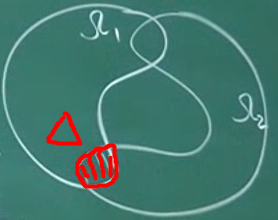
\includegraphics[width=5cm]{assets/04-functions-of-complex-variables/analitical-extension-difinition.png}
    \end{center}

    $f_2$ непосредственное аналитическое продолжение $f_1$ через $\Delta$, если $f_1(z) = f_2(z) \ \forall z \in \Delta$.
\end{definition}
\begin{remark}
    \begin{enumerate}
        \item {
            При фиксации $\Omega_1, \ \Omega_2, \Delta, f_1$, функция $f_2$ определена однозначно.

            \begin{proof}
                $g$ -- непоср. аналитическое продолжение $f_1$:
            
                $g(z) = f_1(z) = f_2(z) \ \forall z \in \Delta$
            
                $g, f_2 \in H(\Omega_2) \underbrace{\implies}_{\text{по т. единственности}} f_2 \equiv g$.
            \end{proof}            
        }
        \item {
            Для другой компоненты продолжение может быть другим (тут понятнее на картинке, добавьте, плиз).
        }
    \end{enumerate}
\end{remark}

\begin{definition}
    $f \in H(\Omega), \ \tilde{f} \in H(\tilde{\Omega})$.

    $\tilde{f}$ -- аналитическое продолжение $f$ на цепочке областей, если $\exists \Omega_1, \dots \Omega_n$ и $f_1 \in H(\Omega_1), \dots , f_n \in H(\Omega_n)$, т.ч. $f_1$ -- непосредственное аналитическое продолжение $f$, $f_2$ -- непосредственное аналитическое продолжение $f_1, \dots, \tilde{f}$ -- непосредственное аналитическое продолжение $f_n$.
    % todo: picture

    \begin{center}
        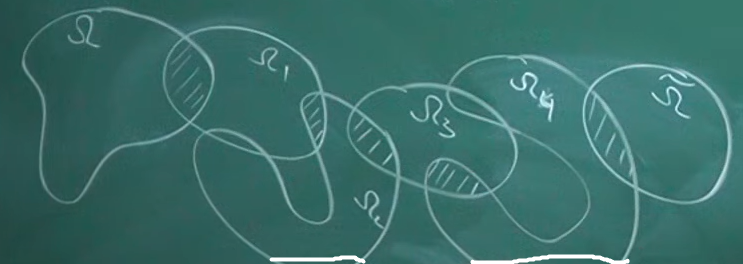
\includegraphics[width=11cm]{assets/04-functions-of-complex-variables/analitical-multiple-extension.png}
    \end{center}
\end{definition}



\begin{remark}
    Рассмотрим всевозможные пары $(f, \Omega)$, т.ч. $f \in H(\Omega)$, тогда существование аналитического продолжения по цепочке областей -- отношение эквивалентности на мн-ве таких пар. 
\end{remark}


\begin{definition}
    Полная аналитическая функция -- класс эквивалентности. 

    $F$ -- полная аналитическая ф-я. $M := \bigcup_{(f, \Omega) \in F} {\Omega}$ -- область определения (существования) $F$.
\end{definition}

\begin{statement}
    $M$ -- область.
\end{statement}
\begin{proof}
    \textbf{Открытость}: объединения открытых -- открытое.

    \textbf{Линейная связность}: $a, b \in M \implies a \in \Omega, b \in \tilde{\Omega}$. $(f, \Omega), \ (\tilde{f}, \tilde{\Omega})$ связана аналитическим продолжением по цепочке, будем переходить по соотвествующим областям и дойдем из $a$ в $b$.
\end{proof}


\begin{definition}
    $F$ -- полная аналитическая функция, $M$ -- область определения $F$, $z \in M$.

    $F(z) := \{ f(z): \ (f, \Omega) \in F \ \land \ z \in \Omega \}$.
\end{definition}

\begin{theorem}
    \textbf{Пуанкаре-Вольтерры}.

    $F(z)$ -- не более чем счетное мн-во.
\end{theorem}

\begin{example}
    $\underbrace{f(z)}_{\frac{1}{1-z}} = \sum_{n=0}^{\infty} {z^n}$ -- ряд сх-ся при $|z| < 1$

    % todo: picture.

    $\frac{1}{1 - z} = \frac{1}{(1-a) - (z - a)} = \frac{1}{1-a} \cdot \frac{1}{1 - \frac{z-a}{1-a}} = \frac{1}{1-a} \cdot \sum_{n=0}^{\infty} { \frac{(z-a)^n}{(1-a)^n} } = \sum_{n=0}^{\infty} { \frac{(z-a)^n}{(1-a)^{n+1}} }$

    $\left| \frac{z-a}{1-a} \right| < 1$ -- круг сходимости ряда.

    $|z-a| < |1-a|$

    % todo: picture
\end{example}


\begin{definition}
    $\sum_{n=0}^{\infty} { c_n \cdot (z - z_0)^n }$, $R$ -- радиус сх-ти ряда.

    % todo: picture

    Берем точку $w$ на границе круга ($|w - z_0| = R$). $w$ -- правильная точка, если найдется $U_w$ -- окр-ть точки $w$ и $g \in H(U_w)$ являющаяся непосредственным продолжением $f$. 
\end{definition}

\begin{definition}
    Особая точка -- точка, не являющаяся правильной. 
\end{definition}

\begin{theorem}
    На границе круга сх-ти лежит хотя бы одна особая точка.
\end{theorem}
\begin{proof}
    От противного. 

    Пусть все точки правильные $|z| = R$ -- правильные.

    $f(z) = \sum_{n=0}^{\infty} { c_n z^n }, \ R$ -- радиус сх-ти.

    $\forall w: \ |w| = R$ -- правильная, тогда найдется $B_{r_w} (w)$ и $g \in H(B_{r_w} (w))$, т.ч. $f = g$ на пересечении $\{ |z| < R \} \cap \{ |z - w| < r_w \}$.

    То есть круги $B_{r_w}(w)$ покрывают окр-ть $|w| = R$. Это компакт, выберем конечное подпокрытие. 

    % todo: picture

    По лемме Лебега $\exists \epsilon > 0: \ B_{\epsilon} (w)$ целиком содержится в элементе подпокрытия.

    $\{ |z| < R + \epsilon \} \subset \{ |z| < R \} \cup$ конечное подпокрытие. 

    $h(z) := \begin{cases}
        f(z), \ |z| < R \\ 
        g_{w_j} (z), \ |z - w_j| < r_{w_j}
    \end{cases} \in H(\{ |z| < R + \epsilon \})$.

    % todo: picture
    $g(z) = \sum_{n=0}^{\infty} { c_n z^n }$ -- ряд Тейлора для $g$, он сх-ся в круге $|z| < R + \epsilon$.

    Противоречие тому, что радиус сходимости был $R$.
\end{proof}

\begin{example}
    \begin{enumerate}
        \item {
            $f(z) = \sum_{n=1}^{\infty} { \frac{z^n}{n^2} }$ сх-ся при $|z| \leq 1$.

            $f'(z) = \sum_{n=1}^{\infty} { \frac{z^{n-1}}{n} }$

            $(zf'(z))' = \sum_{n=0}^{\infty} { z^{n-1} } = \frac{1}{1-z}$
        }
        \item {
            $\sum_{n=0}^{\infty} { z^{2^n} }$ -- сх-ся при $|z| < 1$, все точки $|z| = 1$ -- особые. 
            % todo: picture
        }
    \end{enumerate}
\end{example}


Начало 4-ого семестра.

% Начало 4 семестра
\begin{theorem}
    $f \in H(\Omega)$, \ $\Omega$ -- односвязная, $f \not = 0$ в $\Omega$.

    Тогда существует $g \in H(\Omega)$, т.ч. $e^{g(z)} = f(z)$ и $g$ -- единственна с точностью до аддит. константы $2 \pi i k, \ k \in \mathbb{Z}$.
\end{theorem}

\begin{proof}
    \textbf{Существование}:

    $\frac{f'}{f} \in H(\Omega) \implies $ есть первообразная $g \in H(\Omega)$. 
    
    Подберем константу так, что $e^{g(z_0)} =  f(z_0)$ для некоторого $z_0 \in \Omega$. 

    Покажем, что $g$ подходит: $h(z) := e^{-g(z)} \cdot f(z)$.

    Хотим доказать, что $h \equiv 1$. Знаем, что $h(z_0) = 1$ и
    
    $h'(z) = f'(z) e^{-g(z)} + f(z) e^{-g(z)} (-g'(z)) = e^{-g(z)} \left( f'(z) - f(z) \frac{f'(z)}{f(z)} \right) \equiv 0$.

    \textbf{Единственность}:

    Пусть $e^{g(z)} = f(z) = e^{\tilde{g}(z)} \implies e^{g(z) - \tilde{g}(z)} \equiv 1 \implies \underbrace{g(z) - \tilde{g}(z)}_{\in H(\Omega) \subset C(\Omega)} = 2 \pi i k_{z}: \ k_{z} \in \mathbb{Z} \implies g(z) - \tilde{g}(z) = 2 \pi i k$
\end{proof}

\begin{consequence}
    Пусть $0 \not \in \Omega$ -- односвязна, тогда существует единственный с точностью до $+ 2 \pi i k$ функция $g \in H(\Omega)$, т.ч. $e^{g(z)} = z$.
\end{consequence}

\begin{remark}
    $g(z) = \ln{|z|} + i \arg{z}$
\end{remark}

\begin{remark}
    Обозначение:

    $Ln(z) = \ln{|z|} + i Arg(z)$

    % todo: picture

    ветви логарифма
\end{remark}


\begin{properties}
    \begin{enumerate}
        \item $e^{Ln(z)} = z: \ \forall z \not = 0$
        \item $Ln(z w) = Ln(z) + Ln(w)$
        \item $Ln(z) = \ln{|z|} + i Arg(z)$, где $Arg(z) = \{ \arg{z} + 2 \pi i k: \ k \in \mathbb{Z} \}$
    \end{enumerate}
\end{properties}

\begin{remark}
    Св-во 2 для ветви может быть неверно.

    Берем конкретную ветку и точку:
    % todo: picture
    $0 < \arg < 2 \pi$

    $Ln(-i) = \underbrace{\ln{|-i|}}_{=0} + i Arg(-i) = \frac{3\pi i}{2}$

    $Ln((-i)^2) = Ln(-1) = \ln{|-1|} + i Arg(-1) = \pi i$

    Но $\pi i \not = \frac{3 \pi i}{2} + \frac{3 \pi i}{2}$
\end{remark}

\begin{remark}
    $z^p := e^{p Ln(z)}$ -- полная аналит. функция.

    Если $p \in \mathbb{Z}$, то все однозначно, т.к. $e^{p (2 \pi i k)} = 1$.

    Если $p \in \mathbb{Q}, \ p = \underbrace{\frac{m}{n}}_{\text{несократимая}}$, то $e^{\frac{m}{n} (2 \pi i k)}$ -- принимает $n$ значений.

    Если $p \in \mathbb{C} \setminus \mathbb{Q}$, то $e^{p (2 \pi i k)}$ -- принимает счетное кол-во значений.
\end{remark}



\begin{exerc}
    \begin{enumerate}
        \item Найти $i^i$
        \item Д-ть, что $(z^p)' = \frac{p z^p}{z}$ при $z \not = 0$
        \item $(z w)^p = z^p w^p$ как полные аналитичные функции, но это неверно для ветвей.
    \end{enumerate}
\end{exerc}


\Subsection{Ряды Лорана}

\begin{definition}
    $\sum_{n=-\infty}^{+\infty} a_n (z - z_0)^n$ -- ряд Лорана.

    $\sum_{n = 0}^{\infty} a_n (z - z_0)^n$ -- правильная часть.
    
    $\sum_{n = -\infty}^{-1} a_n (z - z_0)^n = \sum_{n = 1}^{\infty} a_{-n} (z - z_0)^{-n}$ -- главная часть.

    Ряд Лорана сходится $\Leftrightarrow$ правильная и главная части сходятся.
    
    Ниже будем считать, что $z_0 = 0$ для простоты записи.

    $\sum_{n=0}^{\infty} a_n z^n$ -- сх-ся в круге сх-ти $|z| < R$ -- радиус сх-ти $[0, +\infty]$.

    $\sum_{n = 1}^{\infty} a_{-n}z^{-n} = \sum_{n=1}^{\infty} a_{-n} w^{n}$, где $w = \frac{1}{z}$ -- сх-ся в круге сх-ти $|w| < \tilde{R} \implies |z| > \frac{1}{\tilde{R}} =: r$.

    То есть ряд Лорана сх-ся в кольце $r < |z| < R$ -- кольцо сх-ти ряда Лорана.
\end{definition}

\begin{properties}
    \begin{enumerate}
        \item Ряд Лорана абс. сх-ся в кольце $r < |z| < R$, где $r, R \in [0, +\infty]$
        \item В кольце, лежащем строго внутри кольца сх-ти, ряда Лорана сх-ся равномерно.
        \item В кольце сх-ти ряд Лорана можно почленно дифференцировать. 
        \item Ряд Лорана в кольце сх-ти -- голоморфная функция.
    \end{enumerate}
\end{properties}

\begin{theorem}
    Пусть $f(z) = \sum_{n=-\infty}^{\infty} a_n z^n$ в кольце $r < |z| < R$.

    Тогда $a_n = \frac{1}{2 \pi i} \int_{|z| = \rho} {\frac{f(z)}{z^{n+1}} dz}$, где $r < \rho < R$.
\end{theorem}

\begin{proof}
    $\int_{|z| = \rho} { \frac{f(z)}{z^{n+1}} dz } = \int_{|z| = \rho} { \frac{\sum_{k = -\infty}^{+\infty} a_k z^k}{z^{n+1}} dz } =$
    
    $= \int_{|z| = \rho} { \sum_{k=-\infty}^{+\infty} a_k z^{k - n - 1} dz } = \sum_{k = -\infty}^{\infty} a_k \int_{|z| = \rho} { z^{k-n-1} dz } = 2\pi i a_n$

    $\int_{|z| = \rho} { z^m dz } = \int_{0}^{2\pi} { \rho^m e^{i m t} i \rho e^{i t} dt } = \rho^{m+1} i \int_{0}^{2\pi} { e^{i (m+1) t} dt } = \begin{cases}
        2 \pi i, \text{ при } m = -1 \\
        0, \text{ иначе}
    \end{cases}$
\end{proof}


\begin{remark}
    Нер-во Коши тут тоже выполняется:

    $|a_n| \leq \frac{M_{\rho}}{\rho^n}$, где $M_{\rho} = \max_{|z| = \rho}\{ |f(z)| \}$.
\end{remark}

\begin{theorem}
    Пусть $f \in H(r < |z| < R)$. Тогда $f(z) = \sum_{n = -\infty}^{+\infty} a_n z^n$, для некоторых $a_n \in \mathbb{C}$.
\end{theorem}
\begin{proof}
    % todo: picture
    $r < r_1 < r_2 < R_2 < R_1 < R$.

    Берем $r_2 < |z| < R_2$: пишем для него и компакта $K =\{ r_1 \leq |z| \leq R_2 \}$ интегральную теорему Коши:

    $f(z) = \frac{1}{2 \pi i} \int_{\partial K} {\frac{f(\zeta)}{\zeta - z} d\zeta} = \frac{1}{2 \pi i} \int_{|\zeta| = R_1} { \frac{f(\zeta)}{\eta - z} d\zeta } - \frac{1}{2 \pi i} \int_{|\zeta| = r_1} { \frac{f(\zeta)}{\zeta - z} d\zeta }$

    $|\zeta| = R_1, \ |z| < R_2, \ |frac{z}{\zeta}| < \frac{R_2}{R_1} < 1$

    $\frac{1}{\zeta - z} = \frac{1}{1 - \frac{z}{\zeta}} \cdot \frac{1}{\zeta} = \sum_{n=0}^{\infty} { \frac{z^n}{\zeta^{n+1}} }$

    $\int_{|\zeta| = R_1} { \frac{f(\zeta)}{\zeta - z} d\zeta } = \int_{|\zeta| = R_1} { \sum_{n=0}^{\infty} z^n \frac{f(\zeta)}{\zeta^{n+1}} d\zeta } = $

    $= \sum_{n = 0}^{\infty} {z^n \underbrace{\int_{|\zeta| = R_1} { \frac{f(\zeta)}{\zeta^{n + 1}} d\zeta }}_{=: a_n}}$


    $|\zeta| = r_1, \ |z| > r_2, \ |\frac{\zeta}{z}| < \frac{r_1}{r_2} < 1, \ \frac{1}{\zeta - z} = -\frac{1}{z} \cdot \frac{1}{1 - \frac{\zeta}{z}} = -\sum_{n = 0}^{\infty} \frac{\zeta^n}{z^{n + 1}}$

    $-\int_{|\zeta| = r_1} { \frac{f(\zeta)}{\zeta - z} d\zeta } = \int_{|\zeta| = r_1} { \frac{1}{z^{n + 1}} f(\zeta) \zeta^n d\zeta } = $

    $= \sum_{n=0}^{\infty} \frac{1}{z^{n+1}} \underbrace{\int_{|\zeta| = r_1}{f(\zeta) \zeta^n d\zeta}}_{=: a_{n-1}}$
\end{proof}

\begin{theorem}
    Пусть $f \in H(r < |z| < R)$. Тогда существует $g \in H(|z| < R)$ и $h \in H(|z| > r)$, т.ч. $f(z) = g(z) + h(z)$. А если добавить условие: $h \rightarrow_{z \rightarrow \infty} 0$, то такое представление единственно.
\end{theorem}

\begin{proof}
    \textbf{Существование}:

    $f(z) = \sum_{n=-\infty}^{\infty} a_n z^n$.

    Пусть $g(z) = \sum_{n = 0}^{\infty}$ -- главная часть (сх-ся в $\{ |z| < R \}$), $h(z) = \sum_{n = -\infty}^{-1} a_n z^n$ -- правильная часть (сх-ся в $\{ |z| > r \}$).

    \textbf{Единственность}:

    Пусть $f(z) = g(z) + h(z)$, $f(z) = g_1(z) + h_1(z) \implies g(z) - g_1(z) = h_1(z) - h(z)$ при $r < |z| < R$.

    $F(z) := \begin{cases}
        g(z) - g_1(z), \text{ при } |z| < R \\
        h_1(z) - h(z), \text{ при } |z| > r
    \end{cases} \in H(\mathbb{C})$

    Поймем, что $F$ ограничена: $\lim_{z\rightarrow \infty} {F(z)} = 0 \implies$

    $|F(z)| \leq 1$ при $|z| \geq \rho$

    $|F(x)|$ -- огр. при $|z| \leq \rho$ по т. Вейерштрасса.
\end{proof}


